% プロジェクト学習中間報告書書式テンプレート ver.1.0 (utf-8)

% 両面印刷する場合は `openany' を削除する
\documentclass[openany, 11pt,papersize,dvipdfm]{jsbook}

% 報告書提出用スタイルファイル
%\usepackage[final]{funpro}%最終報告書
\usepackage[middle]{funpro}%中間報告書

% 画像ファイル (EPS, EPDF, PNG) を読み込むために
\usepackage{graphicx}
\usepackage{otf}

\def\hissu{\bgroup\color{red}}
\def\endhissu{\egroup}

% ここから -->
%\usepackage{calc,ifthen}
%\newcounter{hoge}
%\newcommand{\fake}[1]{\whiledo{\thehoge<70}{#1\stepcounter{hoge}}%
%  \setcounter{hoge}{0}}
% <-- ここまで 削除してもよい

% 年度の指定
\thisYear{2021}

% プロジェクト名
\jProjectName{``コロナ''に打ち勝つ〜過去から発掘して未来へつなぐ新聞ビッグデータ〜}

% [簡易版のプロジェクト名]{正式なプロジェクト名}
% 欧文のプロジェクト名が極端に長い(2行を超える)場合は、短い記述を
% 任意引数として渡す。
%\eProjectName[Making Delicious curry]{How to make delicious curry of Hakodate}
\eProjectName{Defeating ``COVID-19'' ~ Discovering the past and connecting it to the future - Newspaper Big Data ~}

% <プロジェクト番号>-<グループ名>
\ProjectNumber{12-B}

% グループ名
\jGroupName{グループ~B}
\eGroupName{Group~B}

% プロジェクトリーダ      注意:学籍番号不用
\ProjectLeader{服部俊紀}{Shunki~Hattori}

% グループリーダ      注意:学籍番号不用
\GroupLeader  {日置竜輔}{Ryusuke~Hioki}

% メンバー数
\SumOfMembers{9}
% グループメンバ      注意:学籍番号不用

\GroupMember  {1}{岩上慎之介}{Shinnosuke~Iwagami}
\GroupMember  {2}{田中龍仁}{ Ryuji~Tanaka}
\GroupMember  {3}{保土沢朋和}{Tomowa~Hodosawa}
\GroupMember  {4}{伊藤太一}{ Taichi~Ito}
\GroupMember  {5}{小山内魁人}{Kaito~Osanai}
\GroupMember  {6}{中川翔真}{ Shoma~Nakagawa}
\GroupMember  {7}{金澤快飛}{ Kaito~Kanazawa}



%\GroupMember  {9}{未来敬祐}{Keisuke~Mirai}

% 指導教員
\jadvisor{寺沢憲吾, 美馬のゆり, 角康之, 坂井田瑠衣}
% 複数人数いる場合はカンマ(,)で区切る。カンマの前後に空白は入れない。
\eadvisor{Kengo~Terasawa,Noyuri~Mima,Yasuyuki~Sumi,Rui~Sakaida}

% 論文提出日
\jdate{\today}
\edate{July~16, 2021}

\begin{document}
%
% 表紙
\maketitle

%======================================================================
%前付け
\frontmatter

% 和文概要
\begin{jabstract}
 近年、インターネットメディアの台頭もあり、新聞記事は高い信頼性のある情報が含まれているにもかかわらず、人々に十分に届いていない。また、SNSやスマートフォンの普及などを背景に、デジタルデータは急速に増加している。こうした多様かつ大量のデータを効果的に活用することで、新たな価値を生み出すことが可能となった。そこで、本プロジェクトは、北海道新聞社の協力のもと、過去130年ほどの新聞記事データを活用し、新聞記事をあまり読むことのない人に向け、アクセスする機会を増やすことを目的とした。
活動は、新聞記事の見せ方を工夫するグループAと、新聞記事データを活用した言葉遊びゲームを作るグループ Bに分かれて行っている。
\bunseki{服部俊紀}
 グループBでは、新聞の地域的・歴史的な面に焦点を当て、新聞の記事データから得られる言葉をもとに「クロスワードパズル」や「ヒットアンドブロー」などの言葉遊びゲームを制作する。地方紙が減少し、ニュース砂漠と呼ばれる現象が起こっており、地元の人々が、適切に身近な情報を手に入れる手段が減少している。The New York Times では電子版の新聞にクロスワードパズルを用いることで、新聞の購読者数を安定させた。このように、言葉遊びゲームを通して北海道という地域や時代特有の言葉に触れてもらうことを目的とする。
% 和文キーワード
\begin{jkeyword}
新聞, ビッグデータ, 言葉遊び, 辞書
\end{jkeyword}
\bunseki{小山内魁人}
\end{jabstract}

%英語の概要
\begin{eabstract} The purpose of this project is to use newspaper article data from the past 130 years or so to increase opportunities for people who
currently have little access to newspaper articles. Despite the fact that newspaper articles contain highly reliable information, it is
believed that they are not reaching enough people. Therefore, we will divide into two groups: Group A, which will devise ways to
present newspaper articles, and Group B, which will create games using newspaper article data.\\
Group B will focus on the regional and historical aspects of newspapers, and create word games such as crossword puzzles and hit and blow based on words obtained from newspaper article data. With the decline of local newspapers, a phenomenon known as news deserts, there are fewer and fewer ways for local people to get relevant and accessible information. The New York Times has stabilized the number of subscribers to its electronic version of the newspaper by using crossword puzzles. In this way, the objective of this project is to reconfirm the regional characteristics of newspapers by having participants experience the regional characteristics of newspapers and the unique language of the times through word games.
% 英文キーワード
\begin{ekeyword}
Newspaper, Big Data, Word Play, Data Base
\end{ekeyword}
\bunseki{岩上慎之介}
\end{eabstract}

\tableofcontents% 目次

%======================================================================
\mainmatter% 本文のはじまり

%各章の.texファイルをここに並べる
%ファイル名の「.tex」は省略して良い
\chapter{はじめに}
%該当分野の従来の状況、問題点、本プロジェクトで設定した課題、実施した解決策、及び成果を簡潔に記述する。

\section{プロジェクトの概要}
% 担当:
%プロジェクトの分野の状況や、目的、背景を記述する。 
近年、インターネットメディアの台頭があり、新聞記事は高い信頼性のある情報が含まれているにもかかわらず、人々に十分に届いていない。また、SNSやスマートフォンの普及などを背景に、デジタルデータは急速に増加している。こうした多様かつ大量のデータを効果的に活用することで、新たな価値を生み出すことが可能となった。そこで、本プロジェクトは、北海道新聞社の協力のもと、過去130年ほどの新聞記事データを活用し、新聞記事をあまり読むことのない人に向け、アクセスする機会を増やすことを目的とした。
\bunseki{岩上慎之介}

\section{グループBの概要}
% 担当:
グループB では、新聞の地域的・歴史的な面に焦点を当て、新聞の記事データから得られる言葉をもとに「クロスワードパズル」や「ヒットアンドブロー」などの言葉遊びゲームを制作する。また、地方紙が減少しニュース砂漠と呼ばれる現象が起こっており、地元の人々が適切に身近な情報を手に入れる手段が減少している。The New York Times では電子版の新聞にクロスワードパズルを用いることで、新聞の購読者数を安定させた。そこから発想を受け、言葉遊びゲームを制作し、新聞が持っている地域性や時代特有の言葉に触れてもらい、新聞の持つ地域性を再確認させることを目的として活動を行った。
\bunseki{岩上慎之介}
\chapter{背景}
第2章ではグループ B で調査した新聞の背景について紹介する。新聞の現状における課題点やニュース砂漠、The New York Timesなどの実例を調査した。
\section{現状における問題点}
% 担当:中川翔真
% 背景や目的から現れた問題点を記述する。
グループBでは主に2つの課題が挙げられた。1つ目は、新聞の購読者数が年々減少していることである。特に若者の新聞離れが起きている。2つ目は、地方の新聞紙が無くなるニュース砂漠という現象が起きていることである。ニュース砂漠によって、地方の新聞が減少し、地元の情報を知る機会が減少する。これらの問題から、新聞記事には信頼性の高い情報が含まれているにもかかわらず購読者は減少し続けている。結果として、人々に十分な情報が届かなくなると考えられる。
\bunseki{中川翔真}

\section{実例に対する調査}
% 担当:伊藤太一、小山内魁人
% ニュース砂漠やThe New York Timesの実例に触れた経緯や結果などを記述する。
\subsection{購読者数の推移}
日本新聞協会によると、一般紙とスポーツ紙を合わせ、朝刊夕刊をセットとした発行部数は2000 年では53,708,831部であった[1]。しかし、2020 年では35,091,944 部と約20,000,000 部減少していることが分かった。また、2000 年時点では世帯数が47,419,905 世帯であったが、2020 年では57,380,526 世帯と約10,000,000 世帯増加している(図2.1)。これらの結果から、2000 年では1世帯あたりの部数は1.1 部であるのに対し、2020 年では0.6 部数と約46\%減少していることがわかる。よって、1世帯当たりの部数の減少が問題として挙げられる。\\
 総務省が公開している「主なメディアの利用時間と行為者率」[2]から、若者の新聞に対する関心が薄いと考えられる。総務省のデータをもとに、年代ごとの新聞閲読時間とインターネット利用時間を比較した。グラフ化したものを下記に示す(図2.2、図2.3)。2015年では20代の1日あたりの新聞閲読時間は2.1分であり、2019年での新聞閲読時間は1.8分である。これに対し、2015年の20代の1日あたりのインターネット利用時間は146.9分であり、2019年でのインターネット利用時間は177.7分である。この両者を比較すると、新聞閲読時間はほぼ差がないのに対し、インターネット利用時間は大幅に増加している。また、2015年時点でインターネット利用時間は新聞閲読時間よりも約70倍もの時間である。それに増して2019年では、インターネット利用時間は新聞閲読時間よりも約100倍もの時間である。以上のことから、20代は新聞の利用よりもインターネットの利用に重きを置いている。
\newpage
\begin{figure}[htbp]
    \centering
    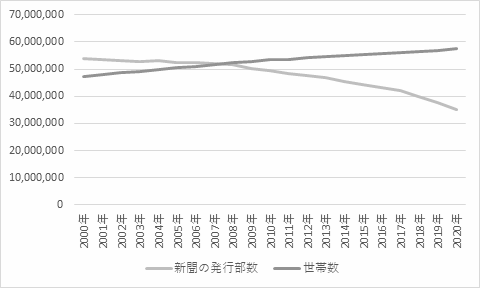
\includegraphics[keepaspectratio, scale=0.5]{images/newspaper1.png}
    \caption{新聞の発行部数と世帯数の推移}
    \label{fig:my_label}
\end{figure}

\begin{figure}[htbp]
    \begin{minipage}[b]{0.45\linewidth}
        \centering
        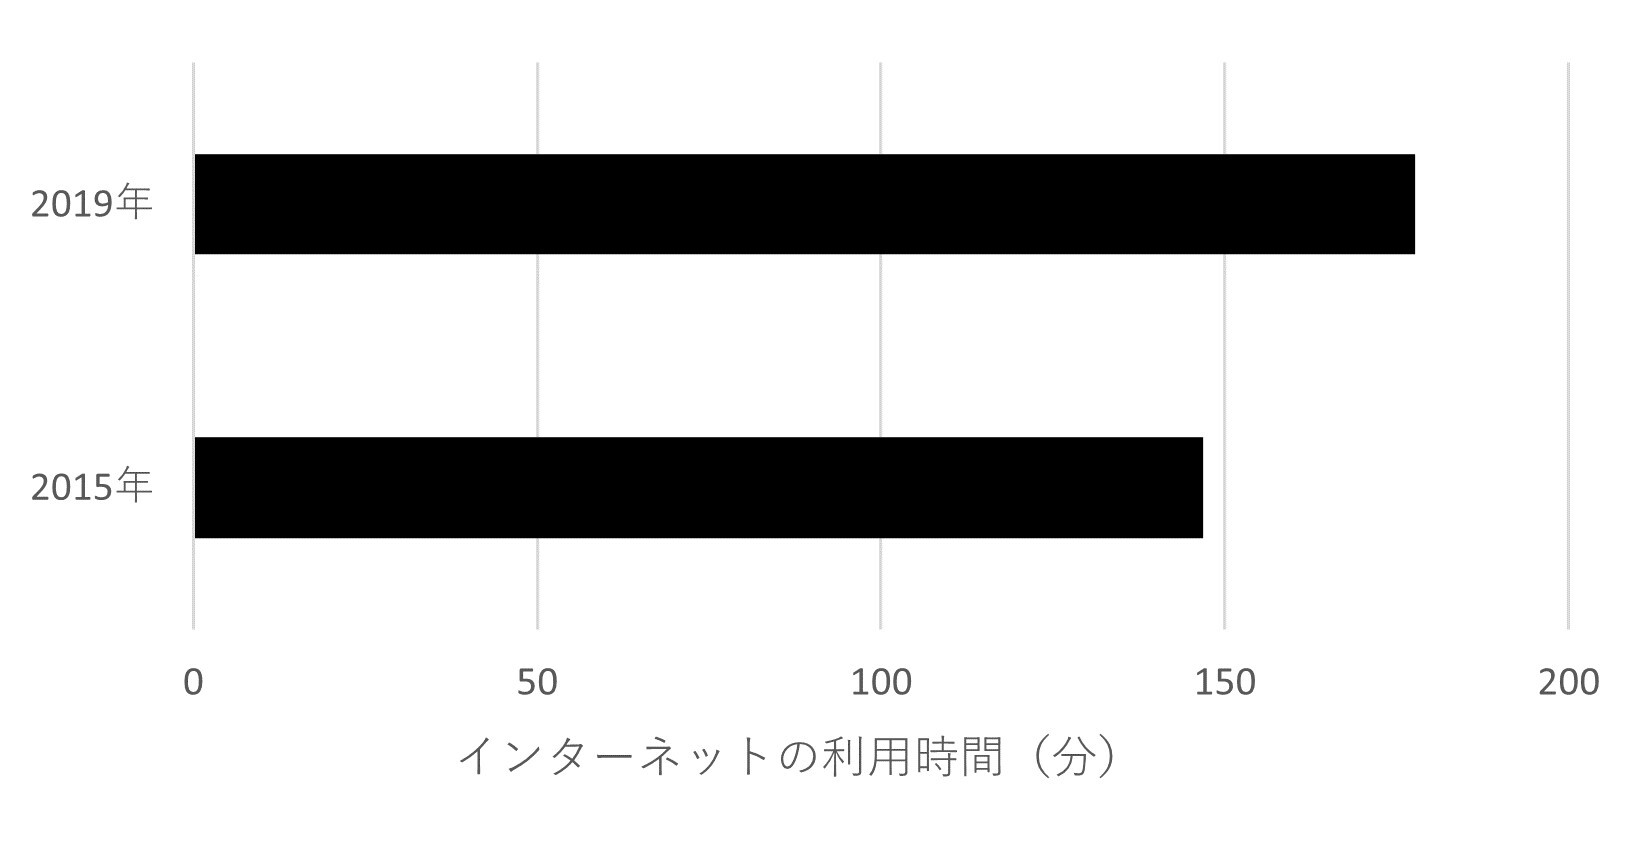
\includegraphics[keepaspectratio, scale=0.5]{images/newspaper2.jpg}
        \caption{20代のインターネットの別利用時間}
    \end{minipage}
    \begin{minipage}[b]{0.45\linewidth}
        \centering
        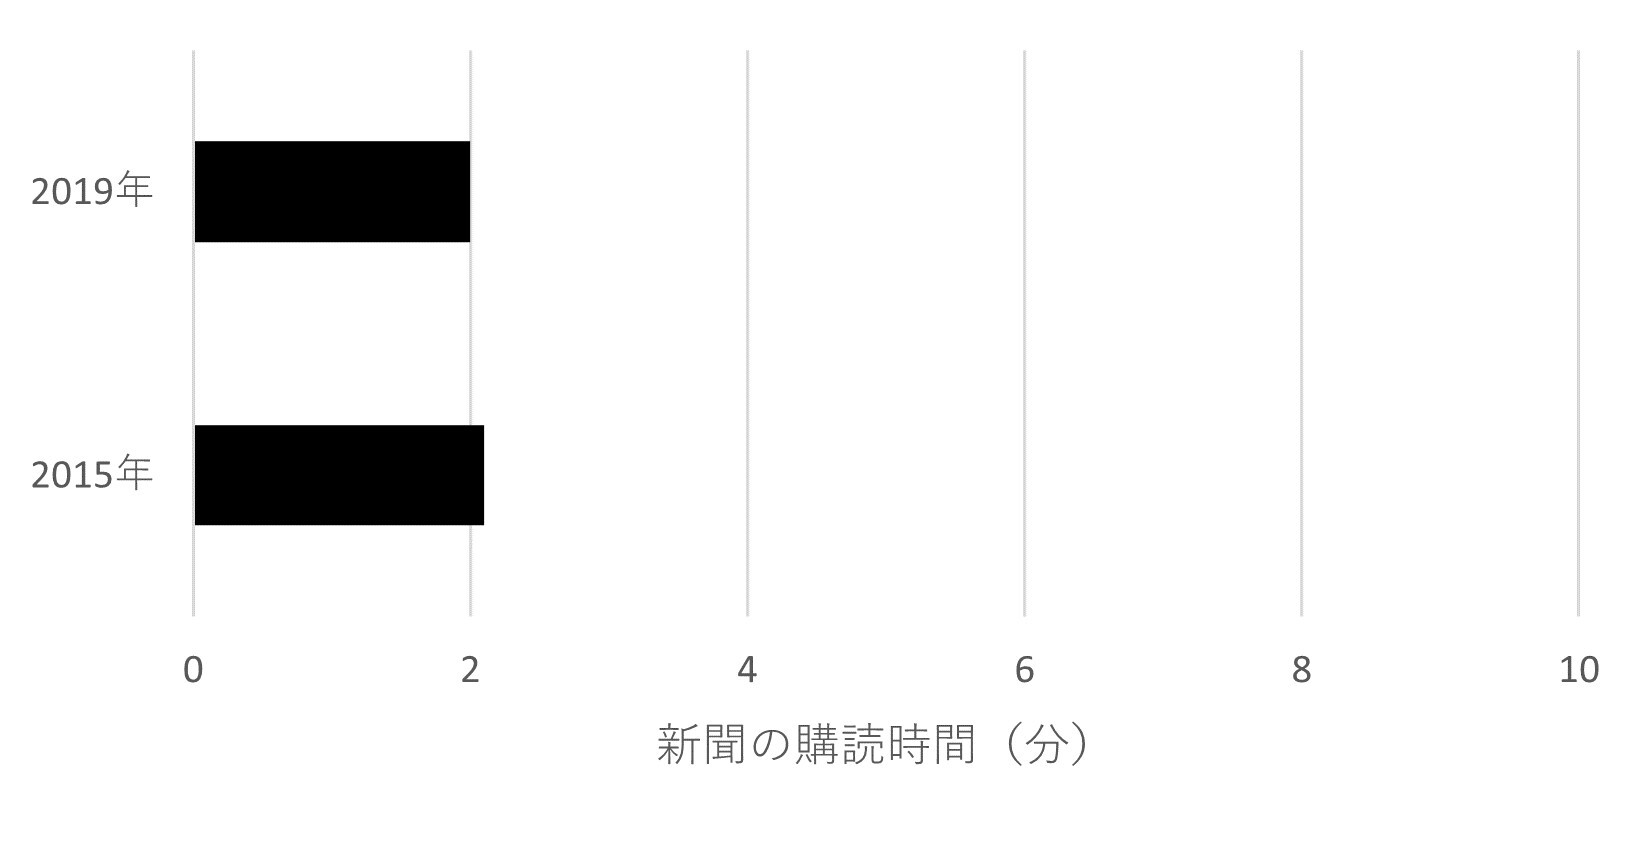
\includegraphics[keepaspectratio, scale=0.5]{images/newspaper3.jpg}
        \caption{20代の新聞の閲読時間 }
    \end{minipage}
\end{figure}
\bunseki{伊藤太一}

\subsection{ニュース砂漠}
ニュース砂漠とは地元に新聞社が0社、または1社であることを指す。実例として、アメリカのノースカロライナ大学の調査によると、アメリカの新聞社のうち 2004 年と比較し 2018 年では 1800 紙が廃刊に追い込まれている。また、ビューリサーチセンターによると2004年から2017年にかけて、新聞社に勤務する記者数が半減している[3]。北海道では、ブロック紙である北海道新聞のほか、函館新聞や旭川新聞などの地方紙が存在する。その一方で2021 年3 月には地方夕刊紙である根室新聞が休刊に追い込まれた[4]。以上より、地方の人々が地元の情報を適切に得ることができなくなっている現状が発見された。
\bunseki{小山内魁人}

\subsection{The New York Times での実例}
The New York Timesでは、電子版のコンテンツとして、クロスワードパズルを導入している。その結果クロスワードパズルを含むコンテンツを目当てとした購読者数が2020年では110万人に達している[5]。
\bunseki{伊藤太一}
\chapter{本プロジェクトにおける目的}
第3章では、グループBでの目的や目的達成のための目標、今後の展望を紹介する。到達目標では、今後制作していくゲームの紹介や、作成する地域・歴史に基づいた辞書の詳細を紹介している。
\section{グループBにおける目的の概要}
% 担当:田中龍仁
% 1.3節で述べた課題をより具体的に記述する。成果に対して必ず満たすべき条件を含む
これらの背景は、新聞がどのようなものであるかを知られていないことが原因の一つであると考えられる。そこで、新聞が持っている地域性や時代特有の言葉に触れてもらい、新聞の持つ特性を再確認させることを目的とする。以上の目的を達成するために、The New York Timesの事例から言葉遊びゲームを利用することとした。そのため、グループBでは、新聞ビッグデータを利用した辞書を活用したゲームを制作するゲーム開発班と、新聞ビッグデータを利用した地域的・歴史的に基づいた辞書を作成する機械学習班の2つに分かれて活動する。
\bunseki{田中龍仁}

\section{到達目標}
\subsection{ゲーム開発班での到達目標}
% 担当:田中龍仁
グループBでは、新聞ビッグデータから抽出した辞書を使用したゲームの制作を目標としている。現段階では、前期の活動を通して「ヒットアンドブロー」、「制限付き言葉遊び」、「新聞クロス」、「文字アナグラム」、「8パズル」、「検索ゲーム」、「きっちり文字埋め」、「シルエット~これなんだろな~」、「センテンスパズル」の計9個のゲームの制作案が出た。
\begin{itemize}
    \item 「ヒットアンドブロー」では、作成した辞書から抽出した言葉を少ない手数で当てるゲームである。文字が入力されると、HIT(文字も場所も正解)の数と、BLOW(文字は正解だが場所が違う)の数が回答される。それをヒントに正解の言葉を当てるゲームを制作する。
\begin{figure}[htbp]
    \centering
    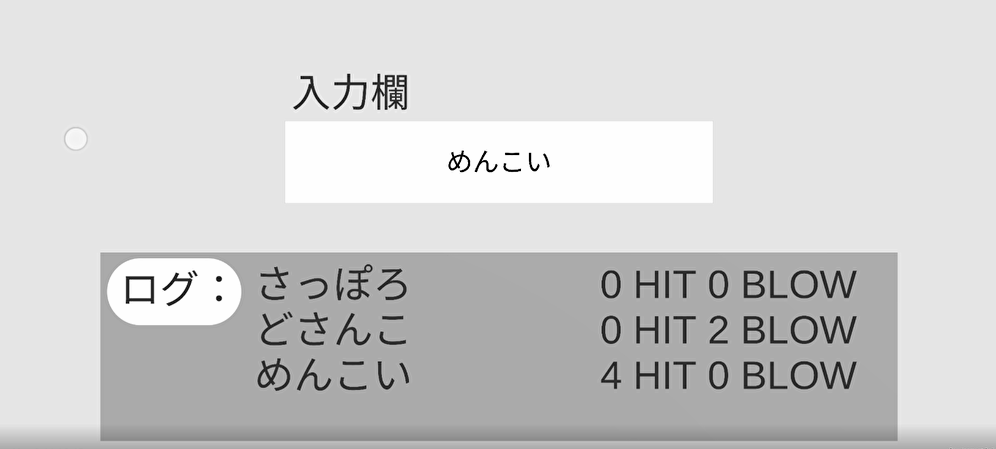
\includegraphics[keepaspectratio, scale=0.3]{images/Project_picuture2.png}
    \caption{「ヒットアンドブロー」の画面}
    \label{fig:my_label}
\end{figure}
\newpage
    \item 「制限付き言葉遊び」では、同じひらがなを2回以上は使えないルールに加えて、さらに時代やお題によって制限された言葉を交互に答え合うゲームを制作する。例えば、50 年前でお題を「北海道の地名」とした場合、「あさひかわ」や「ねむろ」は答えることができる。しかし、「ほくと」を答えてしまうと、北斗市が設置されたのは 2006 年のため使用できない。また、「あさひかわ」と答えた後に次のターンで同じプレイヤが「さっぽろ」を選んでしまうと、「さ」を使用した後にもう一度「さ」を使用しているため、負けとなる。
\begin{figure}[htbp]
    \centering
    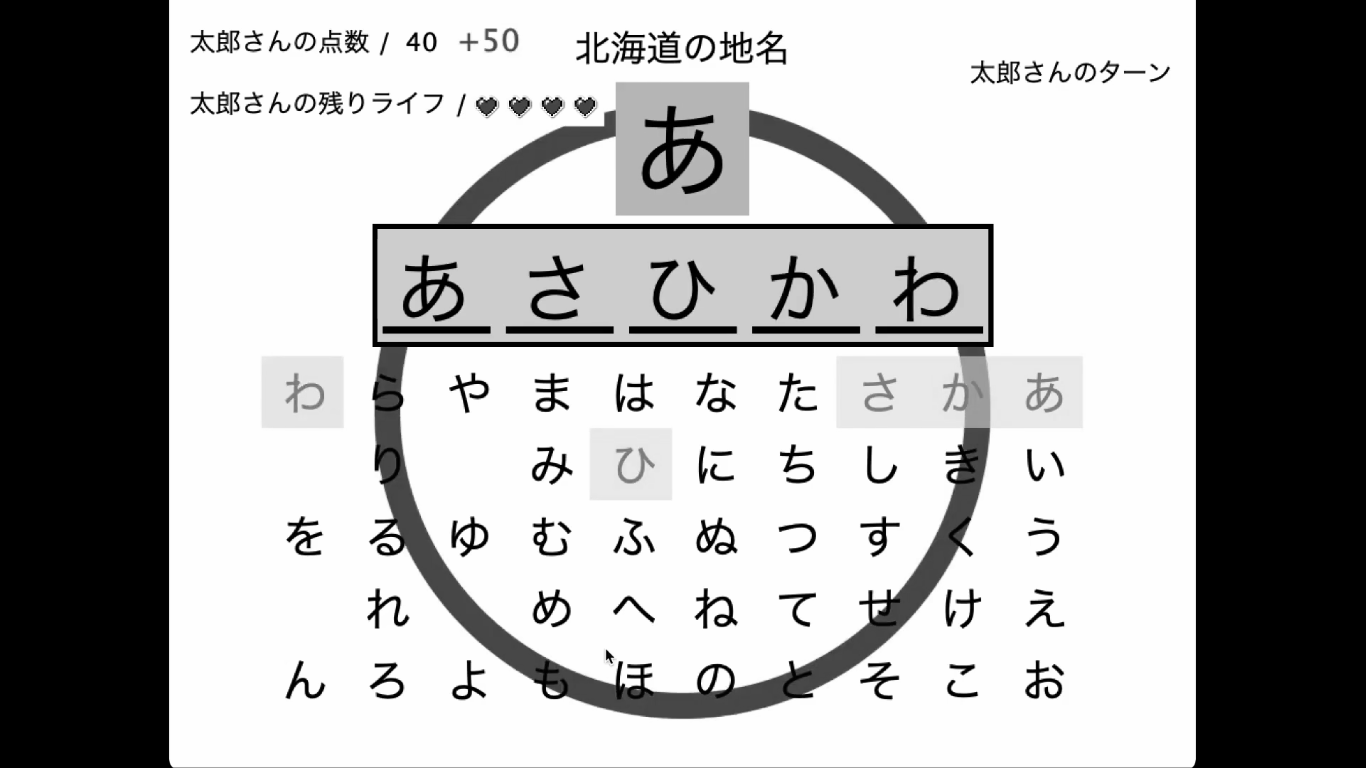
\includegraphics[keepaspectratio, scale=0.2]{images/Project_picuture1.png}
    \caption{「制限付き言葉遊び」の画面}
    \label{fig:my_label}
\end{figure}

    \item 「新聞クロス」では、通常のクロスワードパズルと違い、使われている言葉が北海道に関連したもので作られている。ヒントをもとに、縦・横の文字数に合う言葉を埋めていき、盤面を完成させるゲームを制作する。
\begin{figure}[htbp]
    \centering
    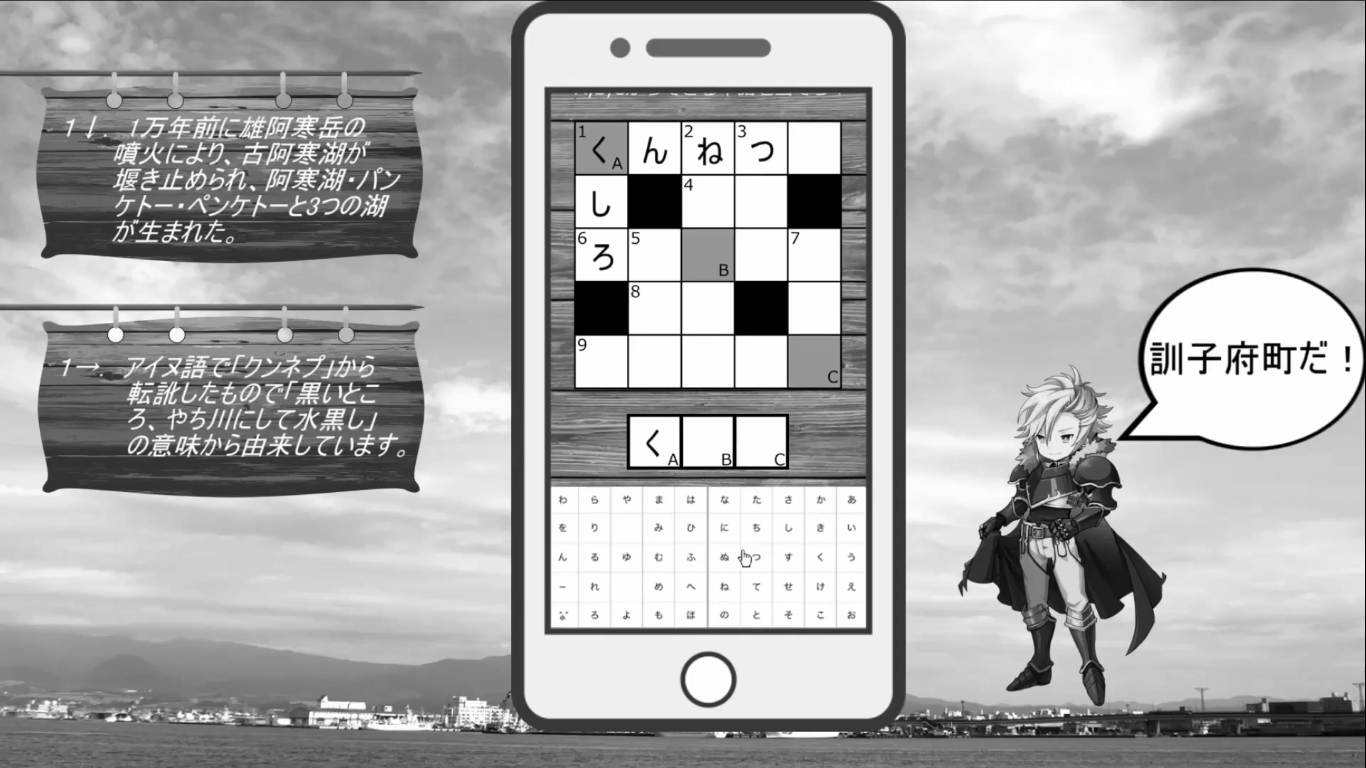
\includegraphics[keepaspectratio, scale=0.2]{images/Project_picuture3.png}
    \caption{「新聞クロス」の画面}
    \label{fig:my_label}
\end{figure}
    \item 「文字アナグラム」では、辞書から抽出した言葉を出題し、出題された言葉をいくつか入れ替えることによって、全く別の意味に変換させるゲームである。例えば、「こさどん」という問題が出題されたとき、文字を入れ替えることで、「どさんこ」という言葉に並び替えることでクリアとなる。\\
    
    \item 「8パズル」では、3×3マスの盤面が用意され、そこには文字の書かれた8つのブロックがある。空白の1マスを利用することで、決められた回数だけブロックを動かしていき最終的により多くの言葉を作るゲームを制作する。\\
    
    \item 「検索ゲーム」では、作成した辞書から北海道に関連した言葉をランダムに抽出し、その言葉がいつの年代の記事に一番現れたかを2人のプレイヤがそれぞれ予想する。予想した年代が一致、もしくは近いプレイヤが勝者となるクイズ形式のゲームを制作する。\\
    
    \item 「きっちり文字埋め」では、新聞の型に収まるように、2人のプレイヤが交互に文字を埋めていく。2人のプレイヤが交互に50音から 1 文字を選び、北海道に関連した言葉を作っていく。決められた手数で多くの言葉を作ることのできたプレイヤが勝利するゲームを制作する。\\
    
    \item 「シルエット~これなんだろな~」では、北海道に関連したシルエットを出題し、そのシルエットが何を表しているか当てるゲームを制作する。例えば、「メロン」のシルエットを出題されたプレイヤはそのシルエットが何を表しているかを予想し、解答する。プレイヤが「メロン」と答えることができたらクリアとなる。\\
    
    \item 「センテンスパズル」では、分解された新聞記事を完成させるために、プレイヤがフィールド上方からランダムに1種類ずつ落下してくる。文字が書かれた片面型テトロミノ状のブロックピースを上手く組み合わせて記事を完成させることで、クリアとなる。\\
    
\end{itemize}
\bunseki{田中龍仁}


\subsection{機械学習班での到達目標}
% 担当:保土沢朋和
新聞ビッグデータを利用した地域・歴史に基づいた辞書の作成を目標としている。地域的側面では北海道に関連した言葉をまとめ、歴史的側面では、それぞれの時代によって使われてきた言葉をまとめる。地域的側面の例としては、「函館」、「長万部」といった北海道の地名や「しゃっこい」、「したっけ」といった方言など、北海道でよく使われる言葉を辞書としてまとめる。歴史的側面の例として、「五稜郭タワー」は 1964 年に建造されたため、それより以前の時代では新聞に「五稜郭タワー」という言葉は存在しない可能性がある。このような、特定の時代には使われているが、それ以前やそれ以降には使われていなかった言葉などを辞書としてまとめる。また、年代ごとに、出現回数の多い言葉や特定の地域ではよく使われている言葉などをまとめることで、ゲーム開発班に提供できるような辞書を作成する。これらのような辞書を作成するために、自然言語処理を用いて開発を行う予定である。
\bunseki{保土沢朋和}

\newpage
\section{今後の展望}
\subsection{ゲーム開発班での開発手段・課題}
% 担当:田中龍仁
ゲーム開発班では、ゲームを開発するにあたってUnityというゲームエンジンを利用する。そこで、Unityを使用するための知識とスクリプトを書く際に使用されるC\#言語の知識の習得が必要である。

\bunseki{田中龍仁}

\subsection{機械学習班での開発手段・課題}
% 担当:保土沢朋和
機械学習班では、新聞ビッグデータを分析するにあたって Pythonを利用する。Pythonとは機械学習の分野で使われるプログラミング言語である。その中で、画像の文字をテキストに変換するために文字認識の知識の習得が必要である。さらに、地域や歴史に基づいた辞書を作成するために自然言語処理や機械学習の知識の習得も必要である。
\bunseki{保土沢朋和}

\section{メンバの割り当て}
% 担当:
グループBではゲーム開発班と機械学習班に分けた。ゲーム開発班は主に成果物であるゲームを作成する班であり、機械学習班はゲームを開発するために使われる新聞データを利用した辞書を作る班である。ゲーム開発班には岩上慎之介、田中龍仁、伊藤太一、小山内魁人、中川翔真の5人が割り当てられた。機械学習班には保土沢朋和、日置竜輔、金澤快飛の3人が割り当てられた。
\bunseki{田中龍仁}
\chapter{前期活動内容}
% 担当:保土沢朋和
第4章ではグループBの活動内容について紹介する。
活動していく中で、意識した点や失敗した要因、その中で身についたことに関して記述している。

\section{完成の理想についての議論}
% 担当:小山内魁人
グループBでは、結成当初、北海道新聞のデータを利用できることから、それを生かした北海道すごろくゲームを考案した。
このゲームは適切な新聞記事をユーザに読ませるマスやミニゲームを行うマスでポイントを競い合うことを想定していた。
また、このゲームは新聞記事データを用いることが目的になっていた。しかし、これらは現状の問題を発見しそれを解決することが目的になっておらず、この成果物はシステム情報科学実習の一環として行うことが不適切であると判断した。
その後、目的と成果物の整合性がとれるように話し合った。
\bunseki{小山内魁人}

\section{新聞の現状の理解}
% 担当:金澤快飛
4.1で各グループメンバでの成果物案を出し合ったが、企画を実現するにあたって必要な根拠が不確かであった。
そこで、各々が調査してきた新聞の現状をGoogle Jamboard内で情報共有し、集約する工程を行った。
Google Jamboardとは、Googleが提供する、リアルタイムで共同作業が可能なホワイトボードのことである(図4.1)。
初期の段階では、情報共有ノートの役割を果たすScrapboxを利用していたが、文字の書き込み以外に適していないという問題があった。
そこで、オンラインでの活動が多かったこともあり、リアルタイム性が高く、文字や図を自由に書き込めるこのシステムを利用するに至った。\\
 情報共有の場では、新聞の購読率の低下が見られ、特に若者の購読者が少ないことがわかった。
その理由としては、購読料が高い、インターネットのような他の媒体がある、読む時間が取れないなどの意見が挙げられた。
一方、スマートフォンやゲームの利用率が一番高いのは若者であることから、新聞とゲームを組み合わせるきっかけとなった。
話し合いを進める中で北海道新聞函館支社長の三浦辰治さんから、アメリカのニューヨークにある新聞社の The New York Times では、電子版の新聞にクロスワードパズルを導入したことにより、購読者数を増加させたという話を聞いた。
\newpage
\begin{figure}[htbp]
    \centering
    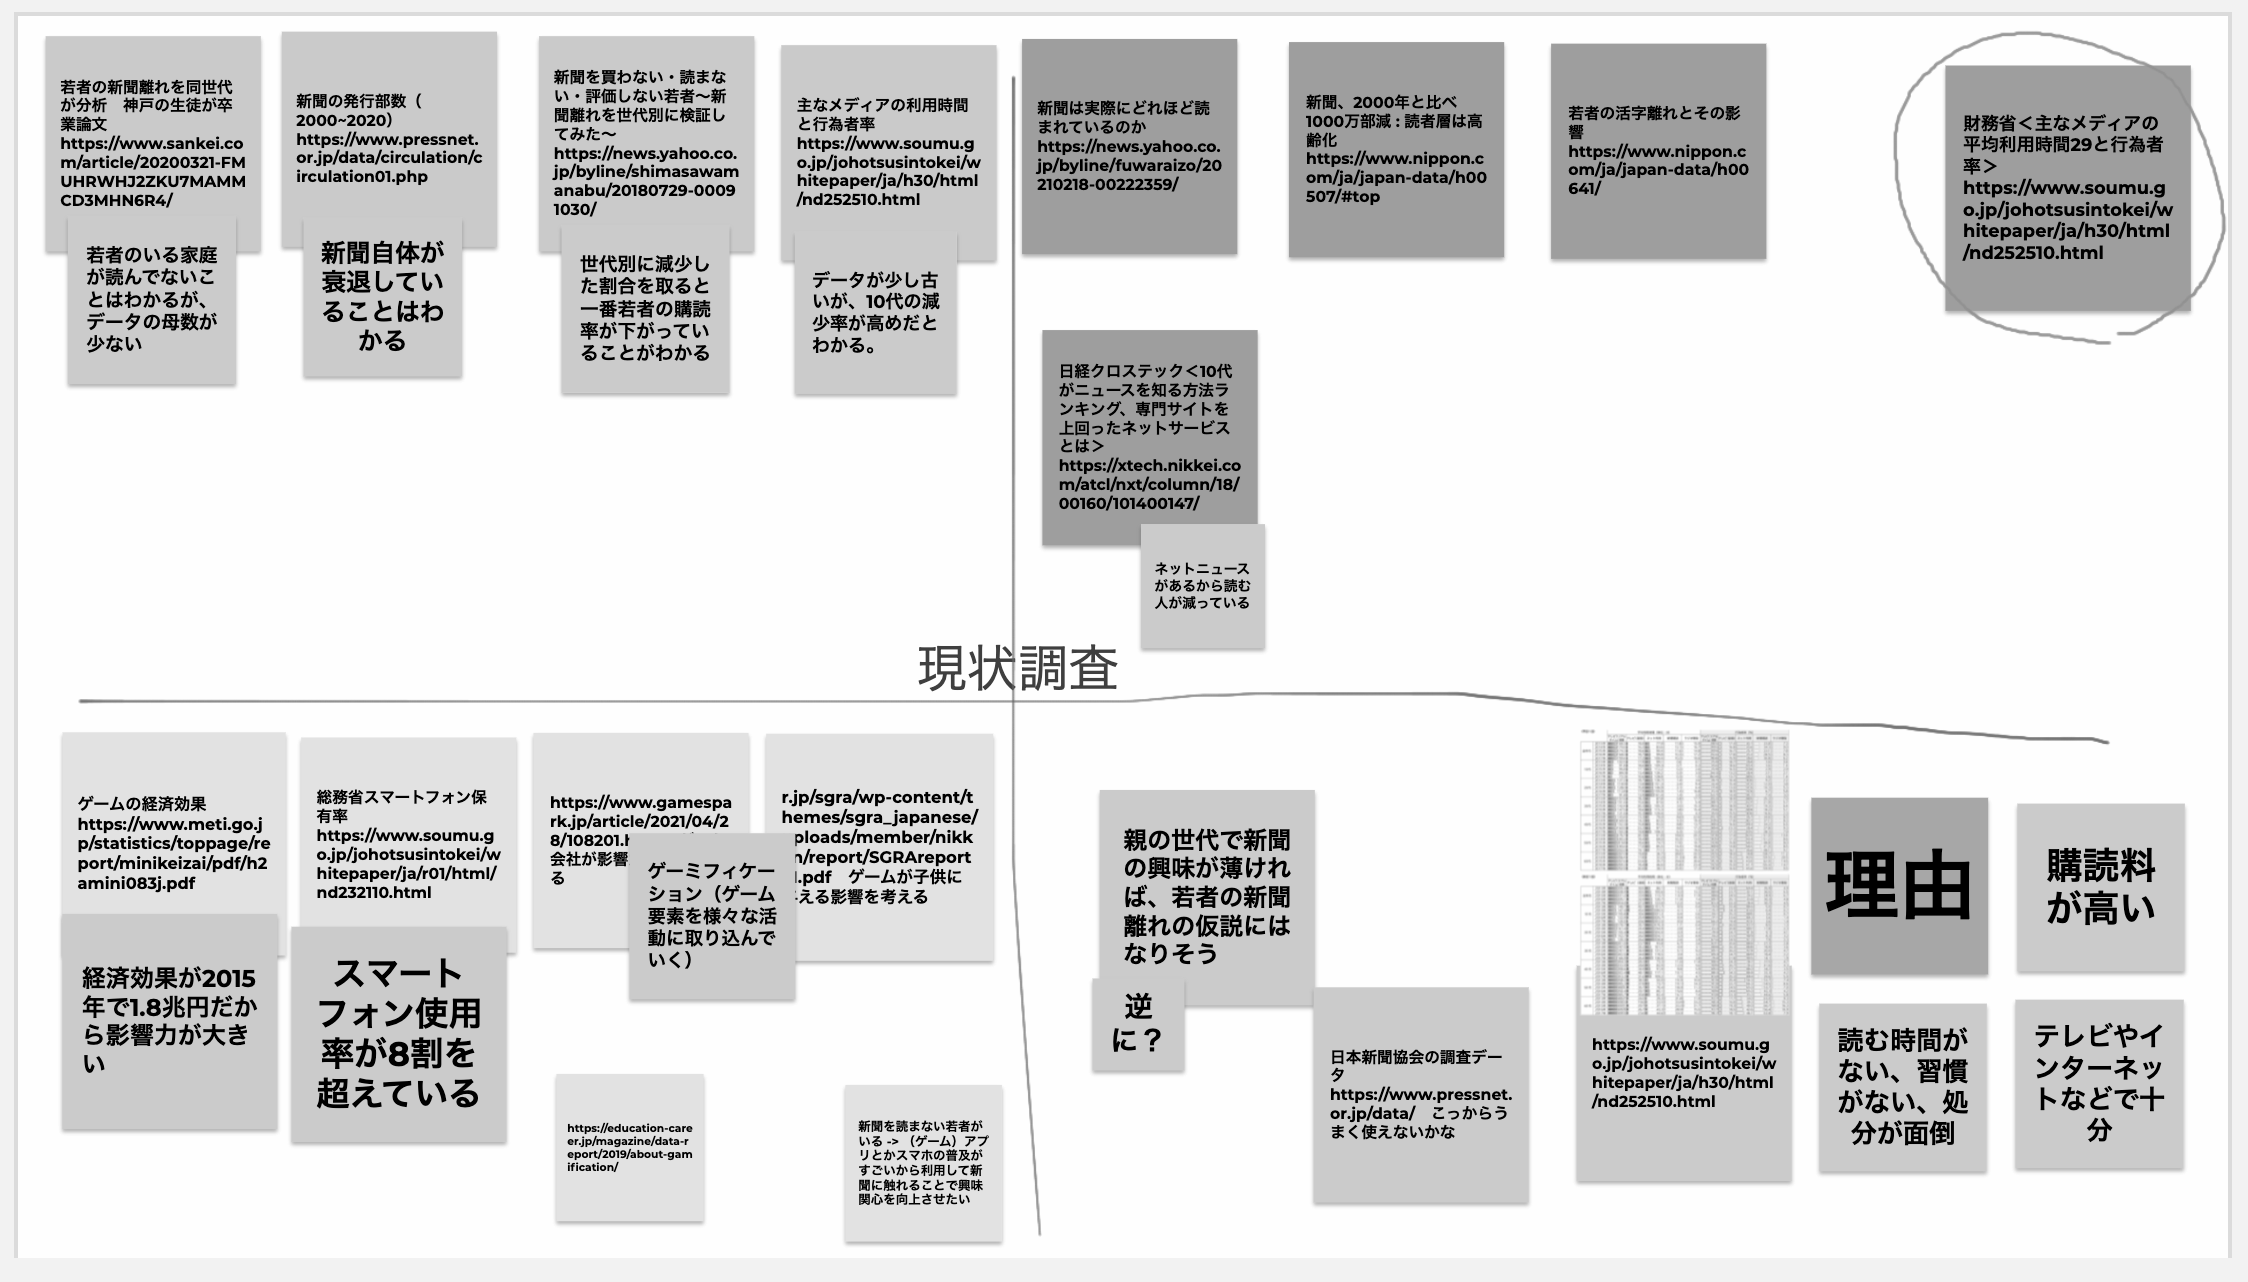
\includegraphics[width=12cm]{images/Project_Research.png}
    \caption{Google Jamboardを使用して背景を共有している様子}
    % \label{fig:my_label}
\end{figure}
\bunseki{金澤快飛}

\section{目的設定}
% 担当:金澤快飛
目的設定は、4.2で挙げられた背景をもとに再度Google Jamboard を利用して話し合った。
初期段階では、背景として若者の新聞における購読率の低下やThe New York Timesがクロスワードパズルの導入により、新聞の購読者を増やしたことから、新聞の購読者数を増やすことを目的として設定していた。
しかし、新聞の購読者数をゲームによって増やすのは、北海道すごろくゲームの際と同様に、目的を達成するのは難しい。
そのため、この目的はシステム情報科学実習の一環として行うことが不適切であると判断した。
そこで、私たちは新聞の特徴である、地域性や歴史性に焦点をあてた。
今回使用する北海道新聞の記事データは、1878 年から2020 年まであり、幅広い年代のものとなっている。
また、ニュース砂漠から、地域的な側面が新聞にあることが読み取れる。\\
 以上より、新聞の持つ地域性に触れてもらうことを目的として設定した。
そのための目標として、新聞ビッグデータをもとに歴史的・地域的な辞書を作成をする。
さらに、作成した辞書をもとに言葉遊びゲームを制作していくこととした。
\bunseki{金澤快飛}

\section{メンバの割り当て}
% 担当:田中龍仁
グループBではゲーム開発班と機械学習班に分けた。
ゲーム開発班は主に成果物であるゲームを作成する班であり、機械学習班はゲームを開発するために使われる新聞データを利用した辞書を作る班である。
ゲーム開発班には岩上慎之介、田中龍仁、伊藤太一、小山内魁人、中川翔真の5人が割り当てられた。
機械学習班には保土沢朋和、日置竜輔、金澤快飛の3人が割り当てられた。
\bunseki{田中龍仁}

\section{ゲーム制作}
言葉遊びゲームを制作するにあたって、各メンバがゲーム案を考え、プレゼンテーションを行った。
その際、共有をしやすいように簡単なゲームやスライドを制作した。
合計9個出たアイデアの中からどのアイデアを採用するか議論していたところ、新たに、すべてのアイデアを採用する案が出てきて、最終的にその案に決まった。
次に、すべてのアイデアをより具体的なものにするため、メンバ全員のアイデアの改善点を話し合った。
中間発表までに、どのゲームのデモンストレーションを制作するかグループ内でアンケートで取った。
その結果、投票数の多かった「制限付き言葉遊び」、「ヒットアンドブロー」、「クロスワードパズル」の3つのゲームのデモンストレーションを制作した。\\
 Unity を利用するのが初めてであり、参考書を読みながら作り上げたので、スクリプトとオブジェクトを繋げる点に苦労した。
また、「ヒットアンドブロー」では、配列を作って入力した文字をログとして表示する点を工夫した。\\
 Processing は学部1 年の頃に使用していたが、文法や基礎知識で欠けている部分があったので、調べながら制作した。
Processing で制作した「制限付き言葉遊び」では、カーソルを文字の上に移動したら強調するホバーの機能をつけて見やすくする点を工夫した。
また、一度使用した文字を2 回目以降は赤く表示させる点においては、配列を用いて実装するのに時間を費やした。
\bunseki{日置竜輔}

\section{デモンストレーション制作}
% 担当:保土沢朋和
中間発表で成果物を掲示するにあたって、デモンストレーションの動画があった方が制作するゲームの内容が伝わりやすいという意見が出たため、4.4で制作した3つのゲームのデモンストレーション動画を作成した。
中間発表で掲示する動画は、約1分程度のものを作成した。
動画作成には、AdobeのPremiere Proを使用した。
Premiere Proを使用するのが初めてであり、インターネットで調べながら作成した。
短期間で3つのゲームのデモンストレーション動画を作成したので時間がかかった。4.4で制作したゲームには、効果音やBGMが無かったのでそれぞれのゲームにあった効果音やBGMを追加した。
さらに、ゲームの内容をより分かりやすく伝えるために、ゲームについての説明を動画に追加した。
\bunseki{保土沢朋和}
\chapter{中間発表}
第5章では、中間発表の準備や発表、講評について紹介する。中間発表で使用するポスターとWebの制作をする際に工夫したことやグループB全体の反省点などをまとめている。
\section{準備・過程}
% 担当:日置竜輔
中間発表では主にポスターとWebの制作について取り組んだ。
ポスター制作に関しては、これまでの活動を説明するだけではなく、より詳細な情報を持っているWebへ誘導する必要があった。初期案では、ゲームのデモンストレーション画面とゲーム全体のUI画面を使用することを考えていた。しかし、ゲーム全体のUI画面は伝えられる情報量が少ないので、削減した。制作途中で、画像を使用する際に元の画像から縦横比を変えたものを使用していたが、元の情報を適切に伝えたり、画像の見栄えを維持するため、元の画像の比率のまま使用することにした。また、行間を広く取った結果、文章量が少なく、情報が少ないものとなってしまった。そのため、行間を狭くし、文章量を多くすることで情報を増やした。
Webの制作に関しては、ポスターと違い、指定された枠組みがないため、出来る限り細かく書いて詳細まで理解してもらえるように取り組んだ。さらに、本文が短く、見出しが画面を埋めてしまうことのないように、イラストや図を用いることで、UIも良くなるように工夫した。また、ゲームのデモンストレーション動画をYouTubeに投稿し、Web内に埋め込むことで具体的にどのようなものを制作する予定なのかを伝える工夫をした。
\bunseki{日置竜輔}

\section{発表}
% 担当:日置竜輔
発表は7月9日金曜日の15:00 - 18:00に Zoom を用いてオンラインで行われた。まず、15:00 - 16:00の1時間を使用し事前に制作したポスター・Webの2つを聴講者に見てもらった後、前半と後半でそれぞれ3つの時間に分かれて質疑応答の時間が設けられた。発表では、事前に司会の進行役や質問の内容に対する回答者を分担していたため、円滑に進行する事ができた。しかし、想定外の観点から質問が来て、答える際に時間をかけてしまい、準備不足を感じる一面もあった。他のプロジェクトでは、質疑応答の時間が終了した後、評価URLを Zoom のチャット欄に貼っていたり、Zoom のカメラの背景をプロジェクトメンバ内で統一していた等、参考に出来る点が多くあった。
\bunseki{日置竜輔}

\newpage
\section{講評}
中間発表終了後に、聴講者の意見が集約したエクセルでのフィードバックを回収した。回収した件数は、37件であり教授が5件、学生が32件であった。また、発表技術の評価、発表内容の評価ともに平均点は7.8378378....(=290/37)点であった。発表内容の評価の中には、「新聞に着目しすぎてビッグデータとの関連性が見られない」といった内容の意見が出ていた。今までグループBおよびプロジェクトとして、新聞との関連性のみを考えていた。グループBは、ビッグデータを多く利用する機会があるため、ビッグデータとの関連性についても今後話し合うことが必要であるとフィードバックを通して意見共有がでた。また、発表技術に関して「質疑時間に詳細に説明していた内容を、公開しているサイトにもう少し記載した方が良い」といった内容の意見があった。他にも質疑応答で、「Webを使用して説明するよりも発表用のスライドを作成して発表した方が良い」といった内容の意見も見られたため、発表で工夫をしていくことが必要である。\\
 講評に関して、課題になるような意見を紹介してきたが、最終成果発表に活かせる意見もあった。例えば、「質問が無い際にグループの説明をした点がよかった」といった内容の意見である。この点に関して、良いと感じたメンバが多数いたため、最終成果発表でも行う予定である。また、「発表者が質問しやすい環境を作ってくれてよかった」といった内容の意見もあった。このような意見を今後参考にする。\\
 グループBでの発表の客観的評価は、5段階中で4段階だとメンバと話し合い決定した。その際に、評価の理由になった項目について記述していく。\\
 はじめに、目的に関してである。目的に関しては、背景との繋がりが弱くまだ協議していくべきであると考えた。 次に、今後の計画の具体性に関してである。今後の計画では、ゲーム制作班ではゲームを、機械学習班ではデータ処理をやることが既に決まっている。そのため、計画の具体性はあるといえる。また、表現力に関しては、ポスターとWebで十分に発揮することができたと考えた。ポスターでは、レイアウトを最優先で作成し、細かい調整も複数回行った。Webでは、デモンストレーション動画を入れることにより、説明のしやすいものにした。また、中間発表で役割分担をすることにより、適切な表現を行うことができた。最後に、チームワークに関してである。チームワークについては、グループメンバ間でタスクを振り分け共有することにより、1人だけ何もしない状況を回避することができた。また、授業時間外でも集まることにより授業内での進行を円滑にすることができた。最終成果発表では、以上の項目を意識するつもりである。
\bunseki{金澤快飛}
\chapter{結果}
\section{プロジェクトの結果}
プロジェクトの結果は、現段階で成果物が完成しておらず評価実験も実施していないため、記述することができない。今後の見通しとしては、ゲームの実装方法や種類について記述する予定である。
\bunseki{伊藤太一}

\section{成果の評価}
グループBの評価は、現段階で成果物が完成しておらずユーザやグループメンバから評価を受けることができない。今後の見通しとしては、ユーザからのレビューや最終成果発表での評価を記述する予定である。
\bunseki{中川翔真}


\newpage
\section{担当分担課題の評価}
%各人の担当課題の成果について、成果によってどのように上述した課題が解決されたか、 要求された役割は果たせたか、残された問題点はあるかを記述する。
\subsection{岩上慎之介}
はじめに、個人としてTeXとゲームの制作の2つを主に行ってきた。TeXでの執筆は初めてで、書き方をグループメンバに教わったり、Webで調べるなどして知識を増やした。グループ報告書制作では、まず章立てを行いそれに伴った執筆担当を決めていった。その後、作成した文章をTexで書きグループ報告書を作成した。\\
 ゲーム開発班としては、ゲームのデモンストレーション段階の制作を課題としていた。現段階では、3つのゲームを制作した。3つのゲームの説明は以下に記述する。
1つ目は、Unityの基礎的な使い方を学ぶため難易度が低い「ブロック崩し」を制作した。Unityの性質やスクリプトとオブジェクトの紐づけに関して学ぶことができた。2つ目は、Unityでの配列の管理とマス目上でのオブジェクトの管理が、成果物を作るうえで良い知識になると考え「五目並べ」を制作した。マス目での入出力の仕方や座標を配列で管理する方法を学ぶことができた。3つ目は、実際にデモ画面を制作するということで、「ヒットアンドブロー」を制作した。配列の管理を学習していたこともあり、莫大な時間をかけず制作することができた。改善点としては、文字を出力する際のアニメーションや効果音の追加などが挙げられる。\\
 今後の課題としてUIの向上や他のゲームの実装、スマートフォンでのデモンストレーションなどが残っている。また、機械学習班で作成した辞書をUnityで使えるように引き継ぐのも重要な課題となっている。現段階で考えているのは、Python for .NETを使用しPythonからC\#にポインタ渡しを行う手段である。機械学習班では、辞書をPythonを使用して作成するため、PythonとC\#で配列を受け渡しする方法が有効である。先ほど記述した手段は、Python for .NETを使用することによりPythonとC\#を同一プロセスで動かすことができる。\\
 今後これらの課題を、ゲーム制作班と機械学習班と話し合いながら解決していくことを目標とする。
\bunseki{岩上慎之介}

\subsection{田中龍仁}
はじめに、グループBで私はゲーム開発班として活動してきた。中間発表案での主な課題として、ゲームのデモンストレーション作成、そして作成したゲームのデモンストレーションを動画として作成することである。グループBでは、9個のゲームを作成しミニゲーム集を作るという目的で活動してきた。まず、どのゲームをデモンストレーションとして作成するか、誰がゲームのデモンストレーションを作成するかを話し合った。その結果、投票結果の多い3個のゲームが候補に挙げられ、それらのゲームのデモンストレーションを作成することになった。私は、ゲーム制作に興味があったので今回は「クロスワードパズル」のデモンストレーション作成に立候補した。この「クロスワードパズル」は、通常のクロスワードパズルと違い、使われている言葉が北海道に関連したもので作られている。そして、ヒントをもとに、縦・横の文字数に合う言葉を埋めていき、盤面を完成させるというルールだ。デモンストレーション段階では各マスへの入力と盤面の作成を目標とした。今回のデモンストレーション作成は、Processingで行った。一番苦労したところは、Processing上でのキーボード作成だ。Processingの実行画面上で表示させるには、自分でオリジナルのキーボードを作るしかなかった。さらに、キーボード上でクリックした文字を各マスに配置するというプログラムを作成することもかなり苦労した。結果として、無事ゲームのデモンストレーションを完成させることができた。また、作成した3個のゲームのデモンストレーションをAdobeのPremiere proで編集し、動画化した。中間発表までの課題だった、ゲームのデモンストレーション作成と動画作成は無事完成させることができた。今後の課題としては、Unityでのゲーム作成、作成したゲームの実装、動画編集技術の向上である。\\
 次にプロジェクト全体の役割としては、私はポスター班としての活動をしてきた。はじめのポスターの構成を考える段階では、Google スライドを使用して話し合いを行った。昨年のプロジェクトのポスターや様々な企業のポスターを参考にし、構成を考えた。構成が完成し、次にポスターに記載する各グループの概要や成果物の説明を考えた。先生方からのたくさんのご指摘を踏まえて、最終的には全員が納得する文章を考えることができた。ここまで、Google スライドを使用して作成していたのだが、イラストや文章の配置がうまくいかずAdobeのInDesignを使用して作成することになった。私は、InDesignの経験がなく、使用方法を勉強することから始めた。不慣れなツールを使用しながらではあったが、中間発表までに納得のいくポスターを完成させることができた。今後の課題としては、InDesignの技術向上とポスター作成に関する知識向上である。
\bunseki{田中龍仁}

\subsection{保土沢朋和}
グループBとして活動を始めた際に、新聞を活かしたゲームについて話し合った。その時に、モンスターを育成するゲームを提案した。このとき私は、とても面白いゲームができると思っていたが、新聞をうまく取り込めておらず、今回のプロジェクトとは少しずれていたため、没案となった。その際、グループ全体に伝えていたものと私が考えていたものが正しく伝わっておらず、没案になる際に自分の考えていたものを正しく伝えることになった。そのため、自分の考えているものを相手に共有するのは容易ではないことを学んだ。その後、先生の助言と話し合いの結果、地域的・歴史的辞書を用いた言葉遊びゲームを作ることになった。その間での話し合いでは意見が没案になったことを引きずってしまい、話し合いで積極的に意見を述べることができていなかった。ここはとても反省すべき点と思っている。\\
 中間発表に向けた制作物はWebを担当した。Webの視認性を高めるために、イラストやグラフを多めに使うことを意識した。ヘッダーの画像を制作し、画像カルーセルに合わせた画像を制作した。Web制作を通じて、視認性についての学習が深まったと思う。\\
 ゲーム班内での分担では機械学習班に振り分けられている。機械学習班は自然言語処理と文字認識の学習を課題としている。現段階で私は、自然言語処理の学習を行っており、10月ごろから始まる開発に向けて準備中である。自分の学習ペースは遅いため、現在からも学習しつつ夏休みからは学習ペースを上げて進めていく予定である。現在の自分の課題としては、自然言語処理と文字認識の知識が乏しく、チームに貢献できていないという点が挙げられるため、これらの学習を迅速に進めていきたい。
\bunseki{保土沢朋和}

\subsection{伊藤太一}
私が主に前期システム情報科学実習で行った活動としては、新聞ビッグデータにかかわる案出し、ポスター制作、グループ報告書の制作である。個人的に力を入れたのは案出しである。このプロジェクトは今年度から発足したことから、過去の成果物に囚われない目標設定が可能であったからである。過去の約130年分の新聞データを活用できる点に着目し、積極的に過去の新聞データを活用できる方法を模索した。明確なグループができる以前は、「新聞擬人化対戦」、「新聞を読んだユーザが何を思い浮かべているかを当てるツール」、「各新聞社の記事を分析し3Dデータ化することによって記事内容の偏りを体感できるツール」などの提案を行った。新聞ビッグデータを活用して言葉遊びゲームを制作するグループBに配属してからは、パズルゲーム、テトリスと新聞ビッグデータを結びつけるゲームを提案し、ゲーム集の1つとして制作することになった。\\
 中間発表にかかわるポスター制作場面においては、文章の背景と目的の文章を作成した。その中でグループのメンバと文章に一貫性があるか、矛盾はないか等の議論をした。また、ポスターデザインに関する情報を調べ、レイアウト、どのフォントを使用すべきか提案した。\\
 グループ報告書の制作場面では、本グループがどのような動機を持って活動するか、その根拠となる背景について調べ、執筆した。総務省が公開している「主なメディアの利用時間と行為者率」と日本新聞協会が公開している「新聞の発行部数と世帯数の推移」の2つのデータをもとに、若者の新聞離れという状況と、新聞業界自体が衰退しているという背景を数字による説明とグラフで可視化した。\\
 前期の個人的な反省点としては、2つある。1つ目は、自分の発言に自信を持てないことが多く、発言する機会を自分自身で減らしてしまったことである。今後このプロジェクトの発展のためには、どんな些細なことでも発言して意見交換することが重要である。2つ目に、ゲーム開発にかかわる技術習得を怠ってしまったことである。このグループで開発に使用するツールは主にUnityというゲームエンジンであるが、このツールは汎用性が高い一方で学ぶべき項目が多い。後期でいざ開発するとなったときに、ツールをある程度使いこなせていないと厳しい。後期で開発に困らないように、今からでも技術習得に向けて学習していく。
\bunseki{伊藤太一}

\subsection{小山内魁人}
主に背景や目的の設定について注力した。背景を調べる際にはより信用できる情報を集めることに気をつけた。また、周りが発信していた様々な情報から、何か新たな発見はないか気を配った。その中で主に3つの背景を調べることができた。1つ目として、新聞の購読者数についてである。新聞の購読者数は年々減っているのではないかという意見が多く、実際に正しいことが分かった。また、これを調べていると、年代別の情報にたどり着くことができ、若者の新聞についての現状を知ることが出来た。2つ目に新聞の信頼性についてである。今では、SNSなど様々、情報伝達方法があることに着目し、それらと新聞とを比較してどのような現状があるかを調べた。その結果、信頼性について、一般の人々が新聞に信頼をおいているということが分かった。3つ目に新聞の現状についてである。新聞は様々な面で問題があることを協力者である北海道新聞函館支社長の三浦辰治さんから情報を受け取っていた。その中で、ニュース砂漠という問題が起こっていることを知ることが出来た。それについて話し合いをしたことで、新聞には地域性という特徴があることに気づくことが出来た。これを通じてこれから活動する背景はどのようなものか、また、どのような方法を用いることで話しあいをスムーズに行うことができるかを学ぶことができた。\\
 目的の設定では、これらの背景をもとに自分たちがどのようなことを成果物を用いて行いたいのかを考える必要があった。はじめに、目的として、新聞の購読者数を増やすという目的を設定した、しかし、この目的は本当に達成可能なのかという指摘をうけて、その後、現在の目的へと変更した。これらから目的の設定の際には、自分たちの成果物が本当にしたいことは何なのかに気を付けて、達成可能であるのか、またそれが何につながるのかなどを考えて設定することを学べた。今後は、ゲーム制作班として活動していく。そのため、これから使用するゲーム開発ツールのUnityや機能の作成に必要なC\#をより深く学んでいく必要がある。
\bunseki{小山内魁人}

\subsection{日置竜輔}
私はグループBのリーダとして前期のシステム情報科学実習を行ってきた。意識して取り組んだことは、効率よく作業を進めていくために全員に仕事を振り分けることである。グループワークを行うにあたり、一人に負担がかかってしまうと作業効率が悪くなってしまうので、一人ひとりに何をしてもらうか常に役割を振るように意識した。その結果、プロジェクト内で決めた期日通りに事を運ばせることができた。私の活動内容としては、前期のシステム情報科学実習で案を練ることはもちろんだが、技術の向上についてもとても力を入れた。\\
 新聞ビッグデータを分析するには、新聞記事を文や単語、品詞ごとに分解する自然言語処理と呼ばれる手法を学習する必要がある。自然言語処理はライブラリが豊富なPythonを用いて学習した。私は、Pythonをある程度学習していたのでスムーズに自然言語処理の勉強に入ることができたが、同じ機械学習班のメンバにはPythonが初めてというメンバがいたので、基礎的な文法や知識を教える活動にも取り組んだ。その結果、私自身は新聞記事をMeCabと呼ばれるモジュールを使用し、品詞ごとに分解して、その出現頻度を可視化したグラフや、北海道に関連した言葉の入った新聞記事を抽出することに成功した。また、Pythonを教えたメンバも文法は理解出来た上に、自然言語処理の基礎を学習できたなどの成果が得られた。\\
 他にも中間発表のWebページで掲載するためのゲームのデモンストレーションを作成するにあたって、Processingを使用し作成した。学部1年の頃に使用していたのである程度は覚えていたが、再度使用すると忘れている部分もあり調べながら実装した。制限付き言葉遊びのデモンストレーションの作成を担当したが、カーソルが文字の上に乗っかることで色を出すホバーの機能などは作成するのにとても苦労した。私は、ゲーム開発班ではないので、機械学習が中心になっていく予定だが、ゲーム開発班が困っていたらサポートしていくつもりである。
後期の活動は実際にビッグデータを全て解析し、実際に言葉遊びゲームの中に分類したデータを渡す必要がある。したがって、さらに細かく解析する、ゲーム開発班の要望に合ったデータを渡すといった内容を後期では取り組んでいくつもりである。
\bunseki{日置竜輔}

\subsection{中川翔真}
このプロジェクトで新聞ビッグデータを見て最初に提案したことが新聞からデータを集め、お料理情報などをまとめることだった。年代やビッグデータを利用して移り変わりやレシピ集、さらにはみやすく提供するものを想定していた。その後全員の案をまとめ、興味を持った分野についての話し合った結果、言葉に着目した。特に回文や名言制作など言葉に関することを追求し、回文探査について具体的な指針を考えた。回文の定義をどうするか、何文字以上の回文が見つかると面白味があるか、文章として成り立つものにするにはどうしたらよいかについて話し合った。次に大まかな3つの班に分かれ、その中で新聞データを調べた。そして、班員と言葉遊びについて話し合った。結果、具体的な成果物が見えず、私が属していた班は解体され、ゲーム班に移籍した。そこで、すごろくとミニゲームという案に加えて、私が元々話していた言葉遊びという案を持ち込んだ。ゲーム班で制作するにあたって背景を調べたところ、The New York Timesがクロスワードパズルで成功している例があり、言葉遊びを中心とするゲームを制作することで決定した。クロスワードパズルやヒットアンドブローなど様々なアプローチから言葉遊びゲームを展開していく中で、私は言葉の読まれ方の変化に目を付けた。シルエットから名前を当てるゲームを提案していたが、アプローチを変え次のようなゲームを提案した。それは、鮭にはシャケやホッチャレなど年代や地域によって様々な呼ばれ方があることを利用したゲームである。\\
 また、中間発表会に向けてポスターの制作を行った。はじめにポスターの内容に関して今まで作業していたスライドの文章を添削した。そのなかで当初話し合っていた私が提案したゲームのタイトル名であるNew Super News paperが採用されそうになっていた。その後は作業が被らないよう、積極的に分担を行い効率よく進めた。そのため、レイアウトを考えるメンバと、文章を考えるメンバに分かれて作業を行った。また、ツールで誤った部分を自分の考えをもとに訂正した。中間発表会では書記をつとめており、質疑応答について正確にメモをとった。今後に活かすために書き方も工夫した。中間報告書の作成では主に背景を担当し、数値を用いてグラフを作成した。後期ではゲーム制作が主な活動になるので、プロジェクトについていけるよう頑張っていきたい。
\bunseki{中川翔真}

\subsection{金澤快飛}
システム情報科学実習の最初の活動として、新聞の特徴やそれに関わる現状の問題を個人で調査した。今まで私は新聞に触れる機会があまり多くはなかった。そのため、この調査では、なぜ新聞が読まれているのか、またなぜ新聞が必要なのかを知ることができ、自分にとって良い機会となった。その後の活動では、新聞記事データを使用して何ができるのかそれぞれがアイデアを考え、発表形式で意見交換を行なった。前期の活動では、特にこのアイデア出し作業にプロジェクトメンバ全員で力を注いだ。活動が進みアイデアが集約していくと本プロジェクトのテーマとして、メディア班とゲーム班に二分されるようになった。私は過去に画像処理について学習していた経験があり、新たなAI技術を習得したいという経緯のもと、ゲーム班内の機械学習班を担当することを選択した。\\
 機械学習班では、新聞ビッグデータの分析、画像データ内文字のテキスト変換、地域性・歴史性のある辞書の作成が課題として挙げられた。これらの課題を達成するためには、プログラミング能力の向上、自然言語処理や機械学習の知識の習得が必要になる。そこで、前期の活動としては主に、本プロジェクトで使用するPython言語や自然言語処理についての学習を行なった。Python言語の学習は、競技プログラミングサイト内の教材を解きながら進めていき、Python言語の特徴や基礎構文について理解することができた。自然言語処理については、実際にプログラムを書きコードを動かしながら自然言語処理を学習することのできる「言語処理100本ノック 2020」[6]というサイトを利用しながら学習を進めていった。このサイトでは、自然言語処理の知識が習得できるだけでなく、プログラミング能力を向上させることができ、効率的学習が可能であることから、今後も続けていこうと予定している。中間発表では、発表資料の素材として、自分が提案した企画と同メンバ一人分のゲームUIの作成をWindows標準ソフトであるペイント3Dを用いて行なった。今後のゲームへの導入を考え、3DモデリングソフトBlenderでのモデリングを想定していたが、期限の制約があり、取り組むことができなかった。そのため、夏休み期間を利用してのモデリング技術の習得も視野に入れている。前期の活動が終了した現在、今後の流れとしては新聞ビッグデータから画像内文字のテキスト変換を行なったのち、テキストデータが詰まったデータベースを作成しようと計画している。そのため、実現に必要な知識の習得、具体的な手法の検討をメンバ間での情報共有・会議などを通して行なっていくつもりだ。
\bunseki{金澤快飛}
\section{今後の予定}
中間発表を終えて、今後改善すべき課題が見つかった。グループBでは、改善すべき課題を踏まえて、下記の予定で活動を行っていく。\\
 8月、9月では、グループメンバで集まり、背景の調査や目的を再確認する。現在調べた背景とグループBのつながりが薄いため、背景の深掘りを行いグループBの目的とのつながりを明確にする。また、機械学習班は画像の文字をテキストに変換するための文字認識の知識や、辞書を作成するために自然言語処理や機械学習の勉強を行う。ゲーム開発班は、ゲームを開発するにあたりUnityやC\#の勉強を行う。具体的には、テキストの扱い方とUIの強化について勉強する。これらを学習する手法として、Webや論文などの参考資料を実際の新聞データに活用して勉強していく。\\
 10月、11月では、それぞれの班に分かれて開発を行う。機械学習班では、自然言語処理を用いて、地域的、歴史的な辞書の作成を行う。また、画像の文字をテキストに変換するために、文字認識を行い開発を進めていく予定である。ゲーム開発班では、機械学習班が作成した辞書を利用し、Unityを用いて言葉遊びゲームの開発を進めていく。その際、Git/Githubを用いた開発を行う予定である。自分たちの成果物について、客観的な意見や感想を集めるために評価実験を行う。\\
 12月では、期末報告書の作成を行う。その際に、発表用スライドの作成など、中間発表で参考になった意見や中間報告書での改善点を活用する。

% 以降、付録(付属資料)であることを示す
\begin{appendix}

% \chapter{新規習得技術}
%課題解決過程に習得した技術について解説する。

%付録の終わり
\end{appendix}

%======================================================================
%\backmatter

% 参考文献
\begin{thebibliography}{9}
 \bibitem{A1} 新聞の発行部数と世帯数の推移, Pressnet 一般社団法人 日本新聞協会,  2021/7/10 アクセス, [online]https://www.pressnet.or.jp/data/circulation/circulation01.php\\
 \bibitem{A2} 第2部 基本データと政策動向, 総務省, 2021/7/10 アクセス, [online]  https://www.soumu.go.jp/johotsusintokei/whitepaper/ja/r02/html/nd252510.html\\
 \bibitem{A3} <フォーカス>米消えゆく地方紙グロスター郡・26自治体に記者1人 「取材してくれぬ」「不正監視弱まる」 北海道新聞(朝刊) 2019年 5月13日\\
 \bibitem{A4} 新聞に載らない内緒話, 長野朝日放送, 2021/7/10 アクセス, [online] https://www.abn-tv.co.jp/naisyo/column/ある「廃刊」/\\
 \bibitem{A5} なぜNYタイムズは新聞のデジタル化に唯一成功した? 紙の売上がまもなく抜かれる, Money Voice, 2021/7/10 アクセス, [online] https://www.mag2.com/p/money/928005\\
 \bibitem{A6} 言語処理100本ノック 2020 (Rev 2), 岡崎直観, 2021/7/16 アクセス, [online] https://nlp100.github.io/ja/
\end{thebibliography}
\end{document}
